\documentclass[../main.tex]{subfiles}
\begin{document}	
    \chapter{Discovery of a cryptic allosteric site in Ebola’s ‘undruggable’ VP35 protein using simulations and experiments}
    \graphicspath{{Chapter5/}}
    \label{ch:vp35pocket}
    \captionsetup{labelfont=bf}
	
    \textit{This chapter is adapted from the following publication:}

    \textit{Cruz, M.A.$^*$ and Frederick, T.E.$^*$, Singh, S., Vithani, N., Zimmerman, M.I., Porter, J.R., Moeder, K.E., Amarasinghe, G.K., and Bowman, G.R., Discovery of a cryptic allosteric site in Ebola's 'undruggable' VP35 protein using simulations and experiments. Preprint on BioRxiv https://doi.org/10.1101/2020.02.09.940510}\cite{Cruz2020vp35}

    \textit{$^*$Authors contributed equally to this work}

    \textit{In this work, my work analyzing the allostery in VP35 and the coupling between the cryptic pocket opening and binding interface is presented in figure \ref{fig:ch5-fig3} and appendix figure \ref{fig:ch5-suppfig2}.}

\section{Abstract}
    Many proteins are classified as ‘undruggable,’ especially those that engage in protein-protein and protein-nucleic acid interactions. Discovering ‘cryptic’ pockets that are absent in available structures but open due to protein dynamics could provide new druggable sites. Here, we integrate simulations and experiments to search for cryptic pockets in Ebola viral protein 35 (VP35). VP35 plays essential roles in Ebola’s replication cycle, including binding the viral RNA genome to block a host’s innate immunity. However, VP35 has so far proved undruggable. Using adaptive sampling simulations and allosteric network detection algorithms, we uncover a cryptic pocket that is allosterically coupled to VP35’s key RNA-binding interface. Experimental tests corroborate the predicted pocket and confirm that stabilizing the open form allosterically disrupts RNA binding. These results demonstrate simulations’ power to characterize hidden conformations and dynamics, uncovering cryptic pockets and allostery that present new therapeutic opportunities.

\section{Introduction}
    Many proteins have proved so difficult to target with small molecule drugs that they are often classified as undruggable, greatly limiting the scope of drug design efforts. In fact, up to 85\% of human proteins have been classified as undruggable because their folds are thought to lack binding pockets where small molecules can bind with the affinity and specificity re{}quired for drug design\cite{hopkins_druggable_2002}. Many undruggable proteins predominantly participate in protein-protein interactions (PPIs) and protein-nucleic acid interactions (PNIs)\cite{arkin_small-molecule_2004,johnson_computational_2017}. In contrast to the binding pockets that many enzymes and receptors use to bind their small molecule ligands, the large flat interfaces involved in PPIs and PNIs do not lend themselves to forming many favorable interactions with small drug-like molecules. As a result, PPIs and PNIs are often considered intractable targets even when there is strong evidence that disrupting these interactions would be of great therapeutic value.

    Cryptic pockets could provide new opportunities to target undruggable proteins\cite{Knoverek:2018kk,vajda_cryptic_2018}, but realizing this potential remains challenging. Such pockets are absent in available experimental structures because they only form in a subset of excited states that arise due to protein dynamics. Cryptic sites can serve as valuable drug targets if they coincide with key functional sites, as can cryptic allosteric sites that are coupled to distant functional sites. However, identifying cryptic pockets remains difficult. Most known cryptic sites were only identified after the serendipitous discovery of a small molecule that binds and stabilizes the open form of the pocket\cite{vajda_cryptic_2018,hardy_searching_2004}. Experimental techniques for intentionally identifying and targeting cryptic pockets show great promise\cite{erlanson_site-directed_2000,ostrem_k-rasg12c_2013,keedy_expanded_2018}, but they still leverage the simultaneous discovery of ligands that bind and stabilize the open pocket. To overcome this limitation, a number of computational methods have been developed to identify cryptic pockets without requiring the simultaneous discovery of small molecules that bind them\cite{Bowman:2012jd,Porter:2019hv,johnson_druggable_2013,oleinikovas_understanding_2016,cimermancic_cryptosite:_2016,schmidt_cosolvent-enhanced_2019,cuchillo_collective_2015,ghanakota_moving_2016}. These methods have proved capable of retrodicting a number of previously identified cryptic pockets. More importantly, applications to a few established drug targets and other enzymes have successfully identified novel cryptic pockets that have been corroborated by subsequent experiments\cite{Porter:2019hv,wassman_computational_2013,schames_discovery_2004}. 

    Here, we integrate atomically-detailed computer simulations and biophysical experiments to explore the potential utility of cryptic pockets in a target that has so far proved undruggable: the interferon inhibitory domain (IID) of Ebola viral protein 35 (VP35). Ebola virus causes a hemorrhagic fever that is often lethal, with case fatality rates approaching 90\% in past outbreaks\cite{keshwara_toward_2017,mulangu_randomized_2019}. While recent progress in vaccine development and use of biologics, such as antibodies, for therapeutic and prophylactic purposes show promise\cite{mulangu_randomized_2019}, small molecule drugs still offer many advantages, including ease of delivery, lower cost, and longer shelf life. The \~120 residue IID of VP35 is a particularly appealing drug target for combating Ebola and other viruses in the Filoviridae family given that it has a well-conserved sequence and plays multiple essential roles in the viral lifecycle\cite{messaoudi_filovirus_2015}. One of its primary functions is to antagonize a host’s innate immunity, particularly RIG-I-like receptor (RLR)-mediated detection of viral nucleic acids, to prevent an interferon (IFN) response and signaling of neighboring cells to heighten their antiviral defenses\cite{cardenas_ebola_2006,basler_ebola_2003,hartman_c-terminal_2004}. Crystal structures have provided a foundation for understanding much about the mechanism of VP35-mediated IFN antagonism\cite{leung_structure_2009,leung_structural_2010}. For example, they have revealed that VP35’s IID binds both the blunt ends and backbone of double-stranded RNA (dsRNA), and that there is a PPI between these dsRNA-binding modes (Fig. \ref{fig:ch5-fig1})\cite{leung_structural_2010}. Disrupting any of these interactions could potentially render Ebola susceptible to a host’s innate immunity. In particular, binding to dsRNA blunt ends plays a dominant role in IFN suppression by Ebola\cite{edwards_differential_2016}. Indeed, mutations that reduce the IID’s affinity for dsRNA blunt ends are sufficient to mitigate IFN antagonism, ultimately attenuating Ebola’s pathogenicity\cite{edwards_differential_2016,hartman_reverse_2006,prins_mutations_2010,prins_basic_2010}. So, disrupting this single binding mode could dramatically reduce the impact of an Ebola infection on the host and potentially reduce deleterious effects, including lethality. However, both dsRNA-binding interfaces are large flat surfaces that are difficult for small molecules to bind tightly (Fig. \ref{fig:ch5-fig1}). As a result, [there are no approved therapies targeting VP35]. Both docking and screening attempts to discover small molecules that bind these interfaces have not yielded sufficiently strong leads to warrant clinical development\cite{brown_silico_2014,glanzer_silico_2016}. The discovery of cryptic pockets in VP35 could provide new opportunities for drugging this essential viral component.

    \begin{figure}[!htb] %Positioning code for figure
        \centering
        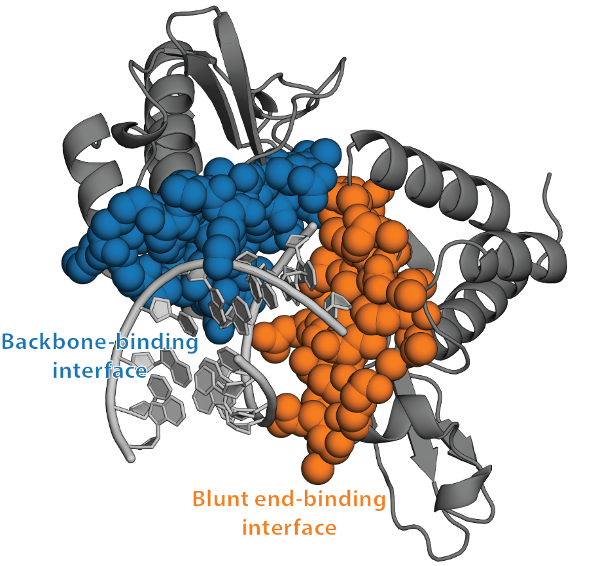
\includegraphics[width=2.5in]{ch5-fig1.png}
        \caption[Crystal structure of two copies of VP35’s IID bound to dsRNA.]
            {Crystal structure of two copies of VP35’s IID (dark gray) bound to dsRNA (light gray) via two flat interfaces (PDB ID 3L25). The backbone-binding interface (blue) and blunt end-binding interface (orange) are shown as spheres to highlight that they lack deep pockets amenable to binding small molecules.}
        \label{fig:ch5-fig1}
    \end{figure}


\section{Results}
    \subsection{Computer simulations reveal a potentially druggable cryptic pocket.}
        We applied our fluctuation amplification of specific traits (FAST) simulation algorithm\cite{zimmerman_fast_2015} to enhance sampling of structures with large pocket volumes that may harbor cryptic pockets. FAST is a goal-oriented adaptive sampling algorithm that exploits Markov state model (MSM) methods to focus computational resources on exploring regions of conformational space with user-specified structural features. An MSM is a network model of a protein’s energy landscape which consists of a set of structural states the protein adopts and the rates of hopping between them\cite{pande_everything_2010,prinz_markov_2011}. Adaptive sampling algorithms enable efficient construction of MSMs by iteratively 1) running a batch of simulations, 2) building an MSM, and 3) selecting a subset of the states that have been identified so far as starting points for the next batch of simulations to maximize the chances of improving the model\cite{bowman_network_2010,Hruska:2018ec}. FAST selects which states to further simulate in a manner that balances exploration/exploitation tradeoffs by considering 1) how well each state optimizes a user defined structural criterion (in this case maximizing the total pocket volume) and 2) the likelihood of discovering new conformational states\cite{zimmerman_fast_2015}. After running FAST, we collected additional simulation data by launching each state on the Folding@home distributed computing environment, which brings together the computing resources of tens of thousands of citizen scientists who volunteer to run simulations on their personal computers. Our final model has 11,891 conformational states, providing a detailed characterization of the different structures the IID adopts but making manual interpretation of the model difficult.

        To identify cryptic pockets within the large ensemble captured by our MSM, we applied our exposons analysis pipeline\cite{Porter:2019hv}. An exposon is a cluster of residues that undergo cooperative changes in their solvent exposure. Coupling between the solvent exposure of every pair of residues is quantified using a mutual information metric, as described in Methods. Exposons are often associated with cryptic sites because the opening/closing of such pockets gives rise to cooperative increases/decreases in the solvent exposure of surrounding residues. Importantly, once an exposon has been identified, our MSM framework provides a facile means to identify the conformational changes that give rise to that exposon.

        The IID has two significant exposons, one of which corresponds to a large cryptic pocket. The blue exposon (Fig. \ref{fig:ch5-fig2}A and \ref{fig:ch5-fig2}B) consists of a set of strongly-coupled residues in helix 7 and adjacent loops and secondary structure elements. Visualizing the conformational change that gives rise to this exposon reveals a substantial displacement of helix 7, creating a large cryptic pocket between it and the helical domain (Fig. \ref{fig:ch5-fig2}C). A number of residues that are displaced along with helix 7 (i.e. A306, K309, and S310) make van der Waals contacts with the dsRNA backbone in the dsRNA-bound crystal structure\cite{leung_structural_2010}, so targeting this cryptic pocket could directly disrupt this binding mode. Retrospective analysis of other validated drug targets suggests cryptic sites created by the movement of secondary structure elements, such as the displacement of helix 7, are often druggable\cite{Beglov:2018dm}. The potential druggability of this cryptic site is also supported by application of the FTMap algorithm\cite{ngan_ftmap:_2012,kozakov_ftmap_2015}, which predicts a number of hotspots within the pocket where small molecules could form a variety of energetically-favorable interactions (\ref{fig:ch5-suppfig1}). Unfortunately, disrupting backbone binding is of less therapeutic utility than disrupting blunt end binding and it is unknown whether the contacts between A306, K309, and S310 are essential for backbone binding. Therefore, it is unclear from this analysis alone whether drugging this newly discovered cryptic pocket would be useful.

        The second exposon (orange in Fig. \ref{fig:ch5-fig2}) encompasses portions of both dsRNA-binding interfaces, but it does not correspond to a cryptic pocket. This exposon includes residues that bind dsRNA’s backbone (i.e. S272) and residues that interact with both the blunt ends and backbone of dsRNA (i.e. F239, Q274, and I340)\cite{leung_structural_2010}. Therefore, altering the conformational preferences of the second exposon could potentially disrupt the blunt end-binding mode and its crucial role in Ebola’s ability to evade an immune response. However, the largest conformational change involved in the formation of this exposon is a displacement of the loop between helices 3 and 4 (Fig. \ref{fig:ch5-fig2}D). This rearrangement does not create a cryptic pocket that is large enough to accommodate drug-like molecules, so it is not obvious how to directly manipulate the orange exposon.

    \begin{figure}[!htb] %Positioning code for figure
        \centering
        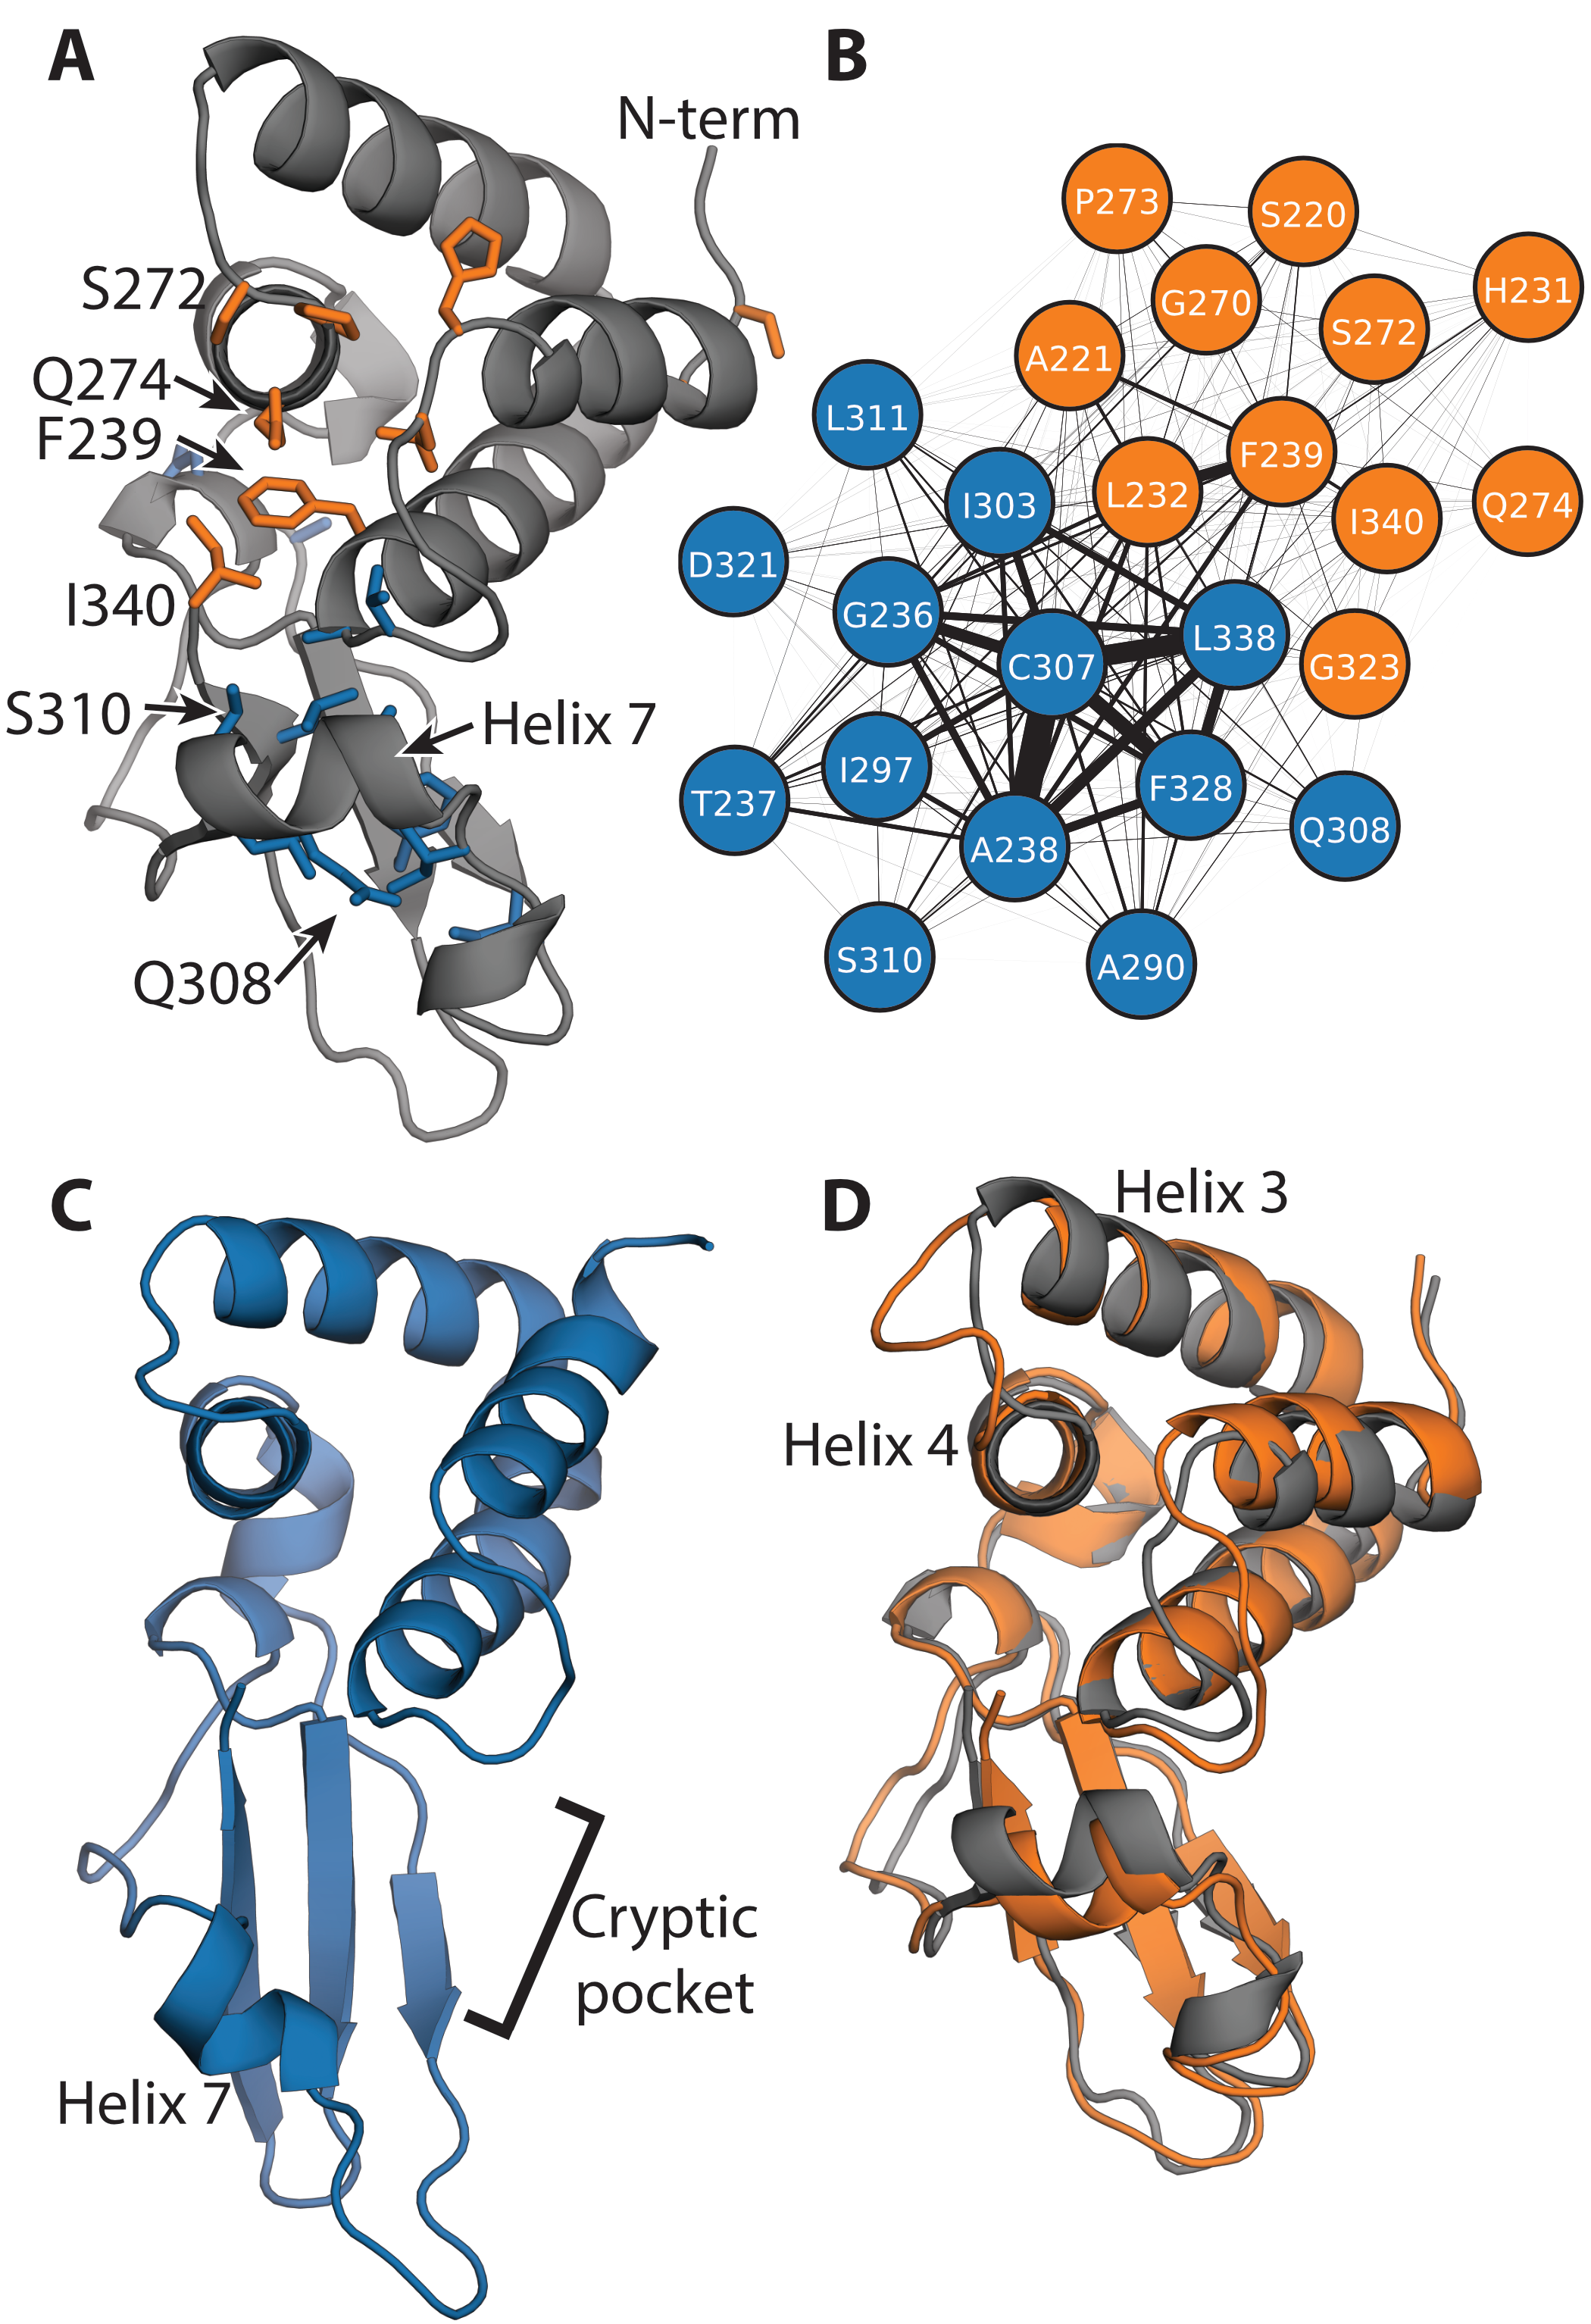
\includegraphics[width=3in]{ch5-fig2.eps}
        \caption[Exposons identify a large cryptic pocket and suggest potential allosteric coupling]
            {Exposons identify a large cryptic pocket and suggest potential allosteric coupling. \textbf{A.} Structure of VP35’s IID highlighting residues in two exposons (blue and orange), the N-terminus (N-term), and C-terminus (I340). \textbf{B.} Network representation of the coupling between the solvent exposure of residues in the two exposons. The edge width between residues is proportional to the mutual information between them. \textbf{C.} Structure highlighting the opening of a cryptic pocket via the displacement of helix 7 that gives rise to the blue exposon. \textbf{D.} Structure highlighting the conformational change that gives rise to the orange exposon overlaid on the crystal structure (gray) to highlight that the rearrangements are subtler than in the blue exposon.}
        \label{fig:ch5-fig2}
    \end{figure}

    \subsection{The cryptic pocket is allosterically coupled to the blunt end-binding interface.}
        Even though the cryptic pocket does not coincide with the interface of VP35’s IID that binds dsRNA blunt ends, it could still serve as a cryptic allosteric site that allosterically controls RNA binding. Indeed, the physical proximity of the two exposons and the coupling between them both hint at the possibility for allosteric coupling. Furthermore, our exposons analysis could easily underestimate this coupling given that it focuses on correlated transitions of residues between solvent exposed and completely buried states, leaving it blind to more subtle conformational fluctuations and the coupling of residues that are always buried (or always exposed). 

        To explore the potential for a broader allosteric network, we applied the correlation of all rotameric and dynamical states (CARDS) algorithm\cite{Singh:2017hh}. CARDS classifies each dihedral in each snapshot of a simulation as being in one of three rotameric states (gauche+, gauche-, or trans) and one of two dynamical states (ordered or disordered). A dihedral is said to be disordered if it is rapidly hopping between different structural states, and it is classified as ordered if it appears to be locked into a single rotameric state for a prolonged time. The mutual information metric is then used to quantify how strongly coupled the structural and dynamical states of each pair of dihedrals are, enabling CARDS to capture the roles of both concerted structural changes and conformational entropy in allosteric communication. Importantly, CARDS accounts for the potential role of residues that are always buried or always exposed to solvent and subtle conformational changes that do not alter the solvent exposure of residues.

        CARDS reveals a broader allosteric network than that identified by our exposons analysis and suggests strong coupling between the cryptic pocket and blunt end-binding interface (Fig. \ref{fig:ch5-fig3}). This network consists of five communities of strongly coupled residues, four of which coincide with large portions of the two dsRNA-binding interfaces. One of these communities (orange) is a hub in the network, having significant coupling to all the other communities. It encompasses part of the orange exposon, particularly residues around the loop between helices 3 and 4. The orange CARDS community and exposon both capture Q274, which engages in both dsRNA-binding interfaces, and S272, which contacts the backbone\cite{leung_structural_2010}. However, the CARDS community includes many additional residues not captured by exposons analysis. Examples include I278, which engages in both dsRNA-binding interfaces, and D271, which is part of the PPI between the two binding modes\cite{leung_structural_2010}. One of the orange community’s strongest allosteric connections is to the green community. This community encompasses the rest of the residues in the orange exposon, including F239 and I340, which are part of both dsRNA-binding interfaces\cite{leung_structural_2010}. The green community also captures additional residues, reaching deep into the helical domain. The orange community is also strongly coupled to the blue community, which includes much of helix 7 and nearby residues that move to give rise to the cryptic pocket that was captured by the blue exposon. Notably, the orange and blue communities are both coupled to a cyan cluster that was not hinted at by our exposons analysis because the residues involved are always solvent exposed. It includes R322, which is part of the blunt end-binding interface and the PPI between the two binding modes, and K282, which also contacts dsRNA blunt ends\cite{leung_structural_2010}. In addition, this community includes K339, which is an important determinant of the electrostatic favorability of dsRNA binding\cite{leung_structural_2010}. Together, these results suggest that opening of the cryptic pocket could strongly impact residues involved in both dsRNA-binding interfaces, as well as the PPI between the two binding modes.

        \begin{figure}[!htb] %Positioning code for figure
            \centering
            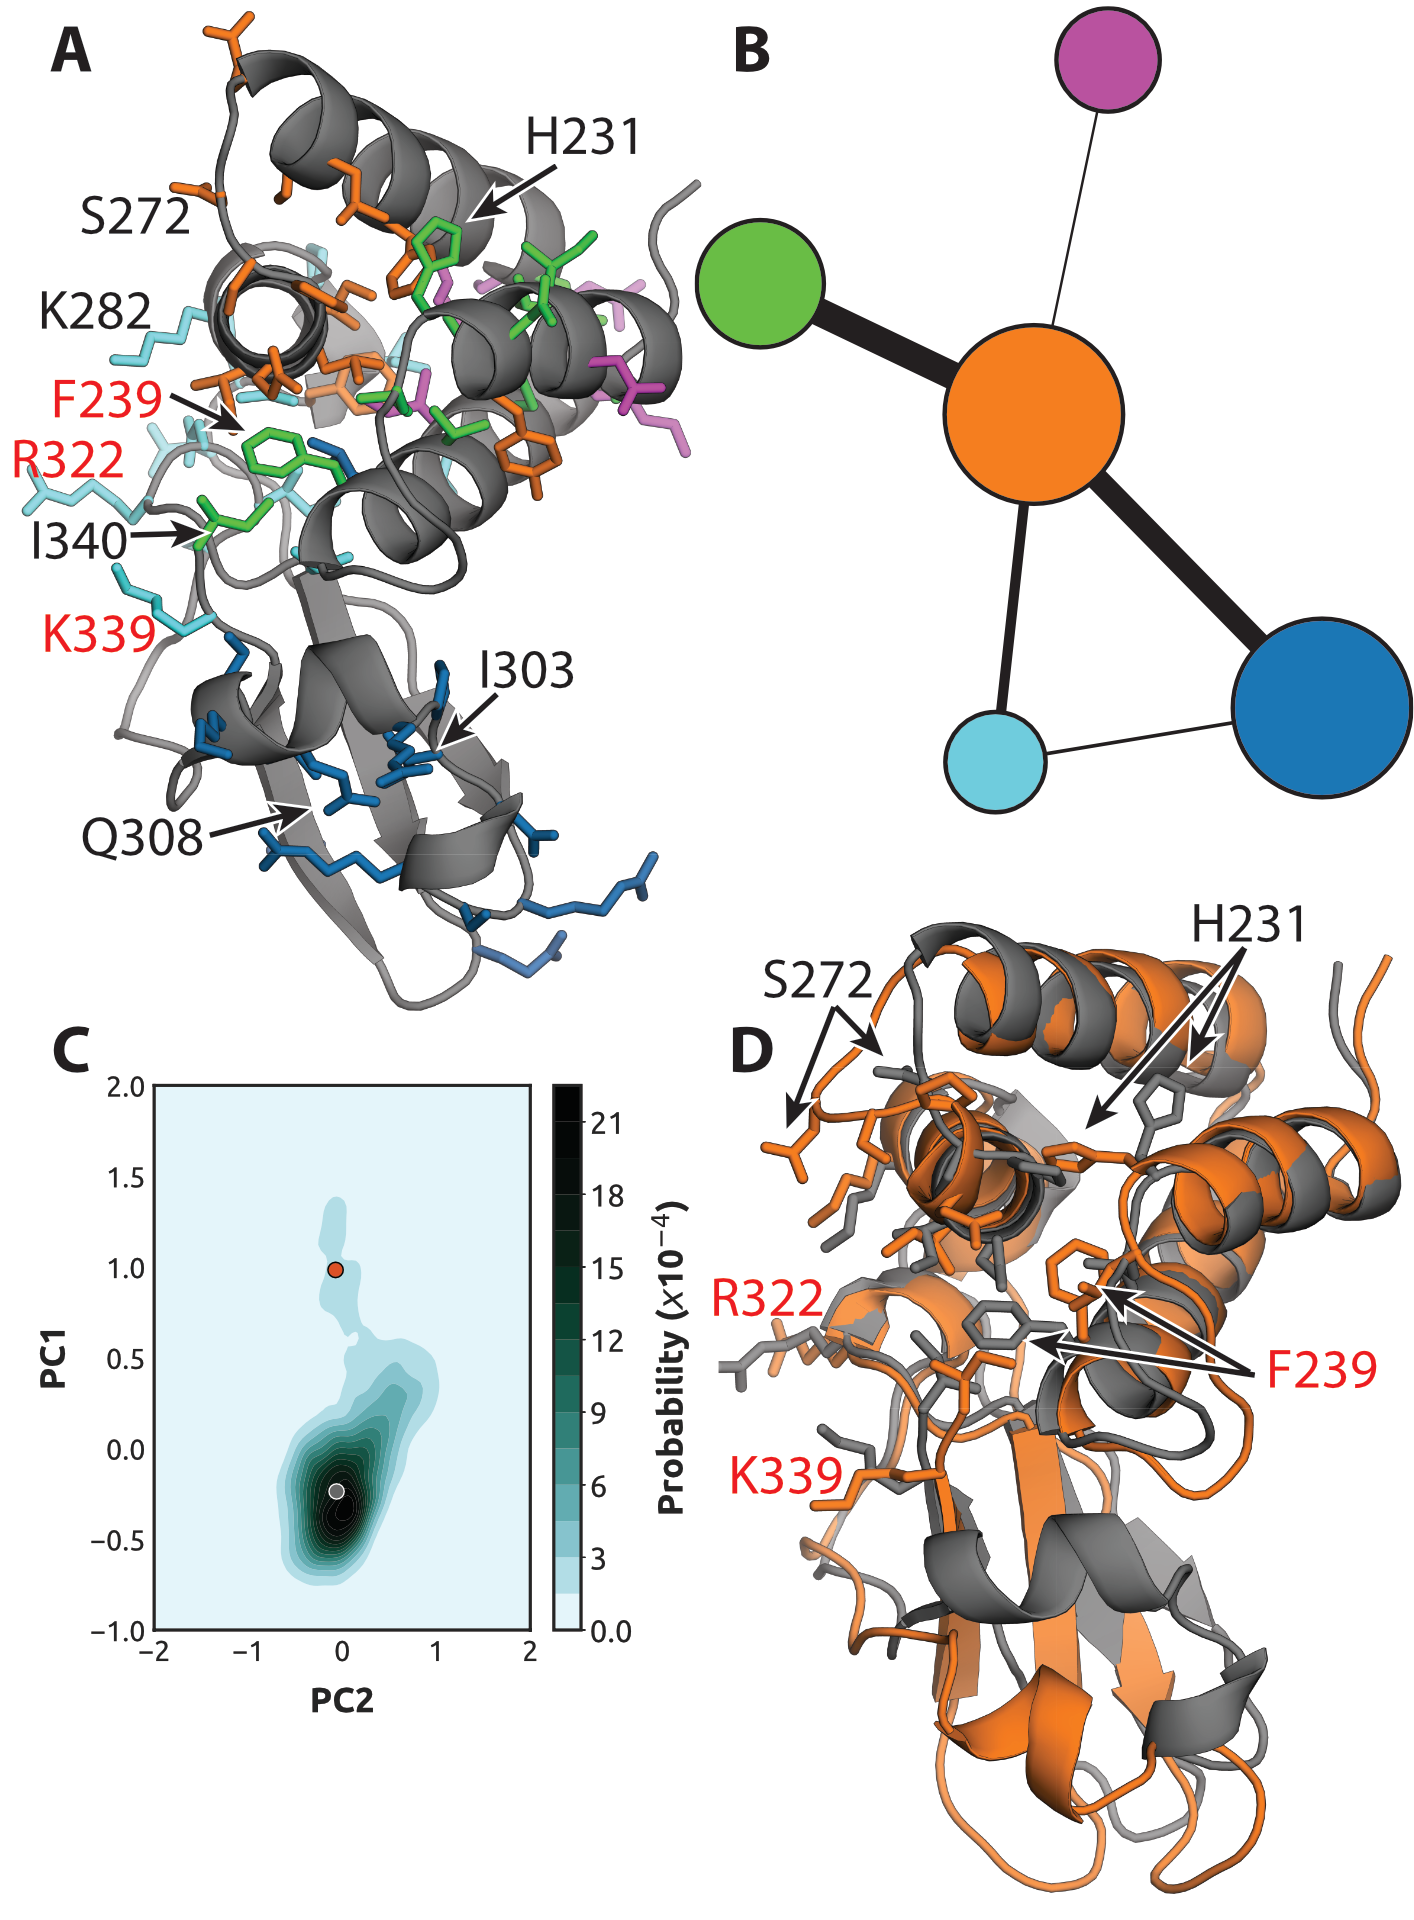
\includegraphics[width=4in]{ch5-fig3.eps}
            \caption[eVP35 allosteric network revealed by the CARDS algorithm]
                {eVP35 allosteric network revealed by the CARDS algorithm. \textbf{A.} Structure of VP35’s IID with residues in the allosteric network shown in sticks and colored according to which of five communities they belong to. Substitution of residues labeled in red with alanine disrupts binding to dsRNA blunt ends and results in a dramatic reduction in immune suppression. \textbf{B.} Network representation of the coupling between communities of residues, colored as in A. Node size is proportional to the strength of coupling between residues in the community, and edge widths are proportional to the strength of coupling between the communities. \textbf{C.} Free energy landscape of the orange exposon projected onto the first two principal components, PC1 and PC2, highlighting the centroid structures of the free energy minimum (gray circle) and excited state (orange circle). \textbf{D.} Structures of the centroids (colored as in panel C) capture opening of the cryptic pocket and rearrangements involving key residues for PPIs and PNIs.}
            \label{fig:ch5-fig3}
        \end{figure}


        To determine the relative importance of the structural and dynamical preferences of this community, we compared the magnitudes of the structural and dynamical components of CARDS. This analysis revealed that concerted structural changes are the dominant mode of allosteric communication in the IID, rather than conformational entropy and dynamical allostery (\ref{fig:ch5-suppfig2}). Therefore, examining structures where the orange community undergoes large conformational changes might reveal the perturbations these motions induce elsewhere in the protein.

        To understand the potential impact of targeting the cryptic pocket on the blunt end-binding mode, we performed a dimensionality reduction based on the orange community. Since the orange community is a hub in the allosteric network, we reasoned that performing a dimensionality reduction based on the structural preferences of this community and examining representative structures would report on what is happening throughout the protein. To understand what sort of conformational changes are present, we performed a dimensionality reduction on our simulation dataset by applying principal component analysis (PCA) to the distances between the C$\beta$ atoms of every pair of residues in the orange community. Projecting our MSM onto the first two principal components (PC1 and PC2) reveals one dominant free energy minimum and a broad excited state (Fig. \ref{fig:ch5-fig3}C).

        Comparing representative structures for the orange community’s two dominant states suggests the cryptic pocket is indeed a cryptic allosteric site, targeting of which could allosterically disrupt binding of VP35’s IID to dsRNA blunt ends. Most importantly, conformational changes of the orange community are associated with opening of the cryptic pocket (Fig. \ref{fig:ch5-fig3}D). Therefore, targeting the cryptic pocket could modulate the entire allosteric network in addition to its potential direct effect on the backbone-binding mode. Comparing the structures also reveals that the end of helix 4 frays and the preceding loop, which sits at the PPI between the two dsRNA-binding modes, is displaced. So, targeting the cryptic pocket could allosterically modulate this PPI. Finally, we note a substantial reshuffling of residues F239, H231, and P273 and modest displacements of R322 and K339. Previous work has demonstrated that F239A, R322A,  and K339A substitutions are each sufficient to disrupt dsRNA binding and IFN suppression\cite{leung_structural_2010}. CARDS analysis suggests targeting the cryptic pocket could allosterically alter the structures of these residues and have a similar impact on dsRNA binding.

    \subsection{Thiol labeling experiments corroborate the predicted cryptic pocket.}
        One way to experimentally test our prediction of a cryptic pocket is to probe for solvent exposure of residues that are buried in available crystal structures but become exposed to solvent upon pocket opening. Cysteines are particularly appealing candidates for such experiments because 1) they have a low abundance and 2) their thiol groups are highly reactive, so it is straightforward to detect exposed cysteines by introducing labeling reagents that covalently bind accessible thiols. Fortuitously, VP35’s IID has two cysteines (C307 and C326) that are buried in available crystal structures but become exposed to solvent when the cryptic pocket opens (Fig. \ref{fig:ch5-fig4}A). There is also a cysteine (C275) that is on the surface of the apo crystal structure\cite{leung_structure_2009} and a fourth cysteine (C247) that is buried in the helical bundle. C275 is typically solvent exposed in our simulations, as expected based on the crystallographic data. Examining the solvent exposure of C247 revealed it is sometimes exposed to solvent via an opening of helix 1 relative to the rest of the helical bundle (\ref{fig:ch5-suppfig3}), but FTMap did not identify any hotspots that are likely to bind drug-like molecules in this region. Therefore, we expect to observe labeling of all four cysteines on a timescale that is faster than global unfolding of the protein.

        To experimentally test our predicted pocket, we applied a thiol labeling technique that probes the solvent exposure of cysteine residues\cite{bernstein_structural_2011}. For these experiments, 5,5’-Dithiobis-(2-Nitrobenzoic Acid) (also known as DTNB or Ellman’s reagent, Fig. \ref{fig:ch5-fig4}B) is added to a protein sample. Upon reaction with the thiol group of an exposed cysteine, DTNB breaks into two TNB molecules, one of which remains covalently bound to the cysteine while the other is released into solution. The accumulation of free TNB can be quantified based on the increased absorbance at 412 nm. We have previously applied this technique to test predicted pockets in $\beta$-lactamase enzymes\cite{Porter:2019hv,Bowman:2015dh}.

        \begin{figure}[!htb] %Positioning code for figure
            \centering
            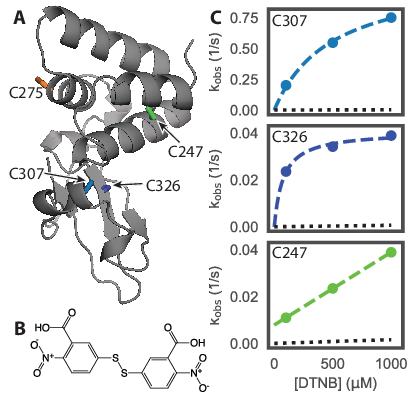
\includegraphics[width=3.85in]{ch5-fig4.eps}
            \caption[Thiol labeling supports the existence of the predicted cryptic pocket.]
                {Thiol labeling supports the existence of the predicted cryptic pocket. Structure of VP35’s IID highlighting the locations of the four native cysteines (sticks). C307 and C326 are both buried and point into the proposed cryptic pocket. B) Structure of the DTNB labeling reagent. C) Observed labeling rates (circles) at a range of DTNB concentrations. Fits to the Linderstrøm-Lang model are shown in dashed colored lines and the expected labeling rate from the unfolded state is shown as black dotted lines. The mean and standard deviation from three replicates are shown but error bars are generally smaller than the symbols. Labeling for C275 is not shown because it is surface exposed in both the available crystal structures and our simulations, and it behaves as expected (labeling rate greater than 1 s$^{-1}$ with a linear dependence on [DTNB]).}
            \label{fig:ch5-fig4}
        \end{figure}

        As expected from our computational model, the observed signal from our thiol labeling experiments is consistent with opening of the cryptic pocket (Fig. \ref{fig:ch5-fig4}C). Absorbance curves are best fit by four exponentials, each with an approximately equivalent amplitude that is consistent with expectations based on the extinction coefficient for DTNB (\ref{fig:ch5-suppfig4}). To assign these labeling rates to individual cysteines, we systematically mutated the cysteines to serines, performed thiol labeling experiments, and assessed which rates disappeared and which remained (\ref{fig:ch5-suppfig6}). For example, labeling of the C275S variant lacks the very fastest rate for wild-type, consistent with the intuition that a residue that is surfaced exposed in the crystal structure (i.e. C275) should label faster than residues that are generally buried. To test whether the observed labeling could be due to an alternative process, such as global unfolding, we determined the population of the unfolded state and unfolding rate of VP35’s IID under native conditions (\ref{fig:ch5-suppfig7}) and the intrinsic labeling rate for each cysteine (\ref{fig:ch5-suppfig6}). As shown in Fig. \ref{fig:ch5-fig4}C, the observed labeling rates are all considerably faster than the expected labeling rate from the unfolded state at a range of DTNB concentrations. This result confirms that labeling of all four cysteines arises from fluctuations within the native state, consistent with our computational predictions. Furthermore, the exposure of C247 is far rarer than C307 or C326 (equilibrium constants for the exposure of C247 and C307 are 5.4×10$^{-4}$$\pm$8.1$\times$10${^-6}$ and 8.5$\times$10$^{-2}$$\pm$2.8$\times$10$^{-3}$, respectively).  Therefore, a ligand would have to pay a greater energetic cost to stabilize the conformational change that exposes C247 than to stabilize the open state of the cryptic allosteric site created by the motion of helix 7.

    \subsection{Stabilizing the open cryptic pocket allosterically disrupts binding to dsRNA blunt ends.}
        We reasoned that covalent attachment of TNB to C307 and C326 would provide a means to capture the open pocket and assess the impact of stabilizing this state on dsRNA binding. Addition of TNB to these cysteines is sterically incompatible with the closed conformation of VP35’s IID that has been observed crystallographically. TNB’s mass of \~198 Da is also similar to many drug fragments used in screening campaigns, making it a reasonable surrogate for the type of effect one might achieve with a fragment hit. Given that we already know DTNB labels the IID’s cysteines, a TNB-labeled sample is easily obtainable by waiting until the labeling reaction goes to completion. Finally, we have previously used this same strategy to identify cryptic pockets that exert allosteric control over the activity of $\beta$-lactamase enzymes\cite{Porter:2019hv,Bowman:2015dh}. To ensure that we primarily capture the effect of labeling on pocket opening, we used a C247S/C275S variant of VP35’s IID that only has cysteines pointing into the cryptic pocket. As with the wild-type protein, thiol labeling of the C247S/C275S variant is consistent with the formation of the proposed cryptic pocket (Supplementary Fig. \ref{fig:ch5-suppfig5}).

        To measure the effect of TNB labeling on the IID’s interaction with dsRNA, we developed a fluorescence polarization (FP) assay for monitoring dsRNA binding. Paralleling our past work on VP35-peptide interactions\cite{liu_sensitive_2017}, we added varying concentrations of C247S/C275S IID to a fixed concentration of 25-bp dsRNA with a fluorescein isothiocyanate (FITC) conjugation at one end (\ref{fig:ch5-suppfig7}). Free FITC-dsRNA emits depolarized light upon excitation with polarized light because of the molecule’s fast rotation. Binding of one or more VP35 molecules restricts the motion of FITC-dsRNA, resulting in greater emission of polarized light, which is best monitored by the change in anisotropy\cite{keck_ssbdna_2012}.

        Monitoring the binding of unlabeled protein to 25-bp dsRNA with either blunt ends or 3’ overhangs demonstrates that our FP assay is sensitive to both dsRNA-binding modes and gives affinities that are consistent with past work. Past work using a dot-blot assay to measure binding reported an apparent dissociation constant (K$_d$) for blunt-ended dsRNA of 3.4$\pm$0.07 $\pm$M\cite{edwards_differential_2016}. Furthermore, sterically hindering binding of the IID to dsRNA blunt ends by adding 2-nucleotide overhangs to the 3’ of the RNA reduces the apparent dsRNA-binding affinity by 10-fold\cite{ramanan_structural_2012}. This weaker interaction was attributed to the backbone-binding mode since it is still available to VP35’s IID even when the presence of an overhang inhibits blunt end binding. Similarly, our FP assay gives an apparent K$_d$ of 3.6$\pm$0.34 $\mu$M for blunt-ended dsRNA (Fig. 5A). Addition of 3’ overhangs results in a strong rightwards shift of the binding curve, consistent with at least a 5-fold reduction in the apparent binding affinity (apparent K$_d$ of 20.4$\pm$1.1 $\mu$M). However, an upper baseline could not be captured due to limitations in the protein’s solubility, so this apparent Kd is a lower bound. The data are also fit well assuming an apparent Kd of 30.1$\pm$7.2 $\mu$M that was reported previously\cite{ramanan_structural_2012}.

        \begin{figure}[!htb] %Positioning code for figure
            \centering
            \includegraphics[width=3.16in]{ch5-fig5.eps}
            \caption[Stabilizing the open cryptic pocket in VP35’s IID disrupts dsRNA binding.]
                {Stabilizing the open cryptic pocket in VP35’s IID disrupts dsRNA binding. \textbf{A.} Binding of both TNB-labeled and unlabeled C247S/C275S variants of the IID to two different dsRNA constructs. This protein variant only has cysteines in the cryptic pocket. The RNA constructs both have a 25-bp double-stranded segment, and one has 2 nucleotide overhangs on the 3’ ends. The anisotropy was measured via a fluorescence polarization assay and fit to a single-site binding model (black lines). The mean and standard deviation from three replicates are shown but error bars are generally smaller than the symbols. \textbf{B.} Circular dichroism (CD) spectra of labeled and unlabeled protein demonstrate that labeling does not unfold the protein. The opaque and semi-transparent lines represent the mean and standard deviation, respectively, from three replicates.}
            \label{fig:ch5-fig5}
        \end{figure}

        Repeating our FP assay with TNB-labeled protein reveals that labeling allosterically reduces the affinity for blunt-ended dsRNA by at least 5-fold (Fig. \ref{fig:ch5-fig5}A). Solubility limitations again prevented us from observing complete binding curves for labeled protein, but the data are sufficient to demonstrate that TNB-labeling has at least as strong an effect on binding as addition of a 3’ overhang. As a control to ensure that labeling does not disrupt binding by simply unfolding the protein, we measured the circular dichroism (CD) spectra of labeled and unlabeled protein. The similarity between the CD spectra (Fig. \ref{fig:ch5-fig5}B) demonstrates that the IID’s overall fold is not grossly perturbed. The slight decrease in helicity at 220 nm can be attributed to the covalent modification disrupting the stability of helix 5 potentially causing local unfolding of this motif. Since the cryptic pocket does not coincide with the blunt end-binding interface, our results suggests the impact on dsRNA binding is allosteric. Furthermore, past work demonstrated that reducing the blunt end-binding affinity by as little as 3-fold is sufficient to allow a host to mount an effective immune response\cite{leung_structural_2010}, so targeting our cryptic pocket could be of great therapeutic value.

\section{Discussion.}
    We have identified a cryptic allosteric site in the IID of the Ebola VP35 protein that provides a new opportunity to target this essential viral component. Past work identified several sites within the VP35 IID that are critical for immune evasion and viral replication\cite{messaoudi_filovirus_2015,hartman_c-terminal_2004,prins_mutations_2010,prins_basic_2010}, but structural snapshots captured crystallographically lacked druggable pockets\cite{leung_structure_2009,leung_structural_2010}. We used adaptive sampling simulations to access more of the ensemble of conformations that VP35 adopts, uncovering an unanticipated cryptic pocket. While the pocket directly coincides with the interface that binds the backbone of dsRNA, it was not clearly of therapeutic relevance since binding dsRNA’s blunt ends is more important for Ebola’s immune evasion mechanism\cite{edwards_differential_2016}. However, our simulations also suggested the cryptic pocket is allosterically coupled to the blunt end-binding interface and, therefore, could modulate this biologically-important interaction. Subsequent experiments confirmed that fluctuations within the folded state of the IID expose two buried cysteines that line the proposed cryptic pocket to solvent. Moreover, covalently modifying these cysteines to stabilize the open form of the cryptic pocket allosterically disrupts binding to dsRNA blunt ends by at least 5-fold. Previous work demonstrated that reducing the binding affinity by as little as 3-fold is sufficient to allow a host to mount an effective immune response\cite{leung_structural_2010}. Therefore, it may be possible to attenuate the impact of viral replication and restrict pathogenicity by designing small molecules to target the cryptic allosteric site we report here.

    More generally, our results speak to the power of simulations to provide simultaneous access to both hidden conformations and dynamics with atomic resolution. Such information is extremely difficult to obtain from single structural snapshots or powerful techniques that report on dynamics without directly yielding structures, such as NMR and hydrogen deuterium exchange. As a result, simulations are a powerful means to uncover unanticipated features of proteins’ conformational ensembles, such as cryptic pockets and allostery, providing a foundation for the design of further experiments. We anticipate such simulations will enable the discovery of cryptic pockets and cryptic allosteric sites in other proteins, particularly those that are currently considered undruggable. Furthermore, the detailed structural insight from simulations will facilitate the design of small molecule drugs that target these sites.

\section{Methods}
    \subsection{Molecular dynamics simulations and analysis}
        Simulations were initiated from chain B of PDB 3L25\cite{leung_structural_2010} and run with Gromacs\cite{VanDerSpoel:2005hz} using the amber03 force field\cite{Duan:2003gt} and TIP3P explicit solvent\cite{Jorgensen:1983fl} at a temperature of 300 K and 1 bar pressure, as described previously\cite{Hart:2016kb}. We first applied our FAST-pockets algorithm\cite{zimmerman_fast_2015} to balance 1) preferentially simulating structures with large pocket volumes that may harbor cryptic pockets with 2) broad exploration of conformational space. For FAST, we performed 10 rounds of simulations with 10 simulations/round and 80 ns/simulation. To acquire better statistics across the landscape, we performed an RMSD-based clustering using a hybrid k-centers/k-medoids algorithm\cite{Beauchamp:2011he} implemented in Enspara\cite{porter2018enspara} to divide the data into 1,000 clusters. Then we ran three simulations initiated from each cluster center on the Folding@home distributed computing environment, resulting in an aggregate simulation time of 122 $\mu$s.

        Exposons were identified using our previously described protocols,11 as implemented in Enspara\cite{porter2018enspara}. Briefly, the solvent accessible surface area (SASA) of each residue’s side-chain was calculated using the Shrake-Rupley algorithm\cite{shrake_environment_1973} implemented in MDTraj\cite{McGibbon:2015fv} using a drug-sized probe (2.8 \AA{} sphere). Conformations were clustered based on the SASA of each residue using a hybrid k-centers/k-medoids algorithm, using a 2.5 \AA{}2 distance cutoff and 5 rounds of k-medoids updates. A Markov time of 6 ns was selected based on the implied timescales test (\ref{fig:ch5-suppfig8}). The center of each cluster was taken as an exemplar of that conformational state, and residues were classified as exposed if their SASA exceeded 2.0 \AA{}2 and buried otherwise. The mutual information between the burial/exposure of each pair of residues was then calculated based on the MSM (i.e. treating the centers as samples and weighting them by the equilibrium probability of the state they represent). Finally, exposons were identified by clustering the matrix of pairwise mutual information values using affinity propagation\cite{Frey:2007hs}.

        The CARDS algorithm\cite{Singh:2017hh} was applied to identify allosteric coupling using our established protocols\cite{Sun:2018kx}, as implemented in Enspara\cite{Singh:2017hh}. Briefly, each dihedral angle in each snapshot of the simulations was assigned to one of three rotameric states (gauche+, gauche-, or trans) and one of two dynamical states (ordered or disordered). The total coupling between each pair of dihedrals $X$ and $Y$ was then calculated as 
        \begin{equation}\label{holistic-mut-inf-eq}
            % \binom{n}{k} = \frac{n!}{k!(n-k)!}
            I_{H}(X_{R},Y_R) = I(X_R,Y_D)+I(X_R,Y_D)+I(X_D,Y_R)+I(X_D,Y_D)
        \end{equation}
         where $I$ is the mutual information metric, $X_R$ is the rotameric state of dihedral $X$, and $X_D$ is the dynamical state of dihedral $X$. The term $I(X_R,Y_R )$ is the purely structural coupling, while the sum of the other three terms is referred to as the disorder-mediated coupling. The dihedral level couplings were coarse-grained into residue-level coupling by summing the total coupling between all the relevant dihedrals. Communities of coupled residues were identified by clustering the residue-level matrix of total couplings using affinity propagation\cite{Frey:2007hs}. The constructed network was subsequently filtered to only retain significant edges\cite{Dianati:2016bt}.These algorithms are available at github.com/bowman-lab. 

    \subsection{Protein expression and purification}
        All variants of VP35’s IID were purified from the cytoplasm of E. coli BL21(DE3) Gold cells (Agilent Technologies). Variants were generated using the site directed mutagenesis method and confirmed by DNA sequencing. Transformed cells were grown at 37°C until OD 0.3 then grown at 18°C until induction at OD 0.6 with 1 mM IPTG (Gold Biotechnology, Olivette, MO). Cells were grown for 15 hours then centrifuged after which the pellet was resuspended in 20 mM Sodium Phosphate pH 8, 1 M sodium chloride, with 5.1 mM $\beta$-mercaptoethanol. Resuspended cells were subjected to sonication at 4°C followed by centrifugation. The supernatant was then subjected to Ni-NTA affinity, TEV digestion, cation exchange (BioRad UNOsphere Rapid S column), and size exclusion chromatography (BioRad Enrich SEC 70 column) into 10 mM Hepes pH 7, 150 mM NaCl, 1 mM MgCl2, 2 mM TCEP. 

    \subsection{Thiol labeling}
        We monitored the change in absorbance over time of 5,5’-dithiobis-(2-nitrobenzoic acid) (DTNB, Ellman’s reagent, Thermo Fisher Scientific). Various concentrations of DTNB were added to protein and change in absorbance was measured in either an SX-20 Stopped Flow instrument (Applied Photophysics, Leatherhead, UK), or an Agilent Cary60 UV-vis spectrophotometer at 412 nm until the reaction reached steady state (\~300 s). Data were fit with a Linderstrøm-Lang model to extract the thermodynamics and/or kinetics of pocket opening, as described in detail previously\cite{Porter:2019hv}. As a control, the equilibrium constant for folding and the unfolding rate were measured (\ref{tab:ch5-supptab1}) and used to predict the expected labeling rate from the unfolded state. The equilibrium constant was inferred from a two-state fit to urea melts monitored by fluorescence and unfolding rates were inferred from single exponential fits to unfolding curves monitored by fluorescence after the addition of urea, as described previously\cite{Porter:2019hv,Bowman:2015dh,zimmerman_prediction_2017}. Fluorescence data were collected using a Photon Technology International Quanta- Master 800 rapid excitation spectrofluorometer with Quantum Northwest Inc. TC-125 Peltier-controlled cuvette holder. 

    \subsection{Fluorescence polarization binding assay}
        Binding affinities between variants of VP35’s IID and dsRNA were measured using fluorescence polarization in 10 mM Hepes pH 7, 150 mM NaCl, 1 mM MgCl2. A 25 base pair FITC-dsRNA (Integrated DNA Technologies) substrate with and without a 2 nucleotide 3’ overhang was included at 100 nM. The sample was equilibrated for one hour before data collection. Data were collected on a BioTek Synergy2 Multi-Mode Reader as polarization and were converted to anisotropy as described previously\cite{keck_ssbdna_2012}. TNB-labeled samples were generated by allowing DTNB and VP35’s IID to react for 3 minutes and then removing excess DTNB with a Zeba spin desalting columns (Thermo Fisher Scientific). A single-site binding model was sufficient to fit the data.

\section{Acknowledgements}
    We are grateful to the citizen scientists who participate in Folding@home for volunteering to run simulations on their personal computers. This work was funded by NSF CAREER Award MCB-1552471 and NIH grant R01 GM124007 (Bowman), as well as NIH grants R01AI123926, P01AI120943, and R01AI143292 (Amarasinghe). GRB holds a Career Award at the Scientific Interface from the Burroughs Wellcome Fund and a Packard Fellowship for Science and Engineering from The David \& Lucile Packard Foundation. MAC was supported by the 5R25GM103757 IMSD program and SS was supported by a MilliporeSigma Fellowship. We thank Drs. Timothy M. Lohman and Alexander G. Kozlov for advice on FP assays. 

% \section{Supplementary Material} 
    % \renewcommand{\thefigure}{\arabic{chapter}.S\arabic{figure}}
    % \setcounter{figure}{0}

%     \begin{figure}[!htb] %Positioning code for figure
%         \centering
%         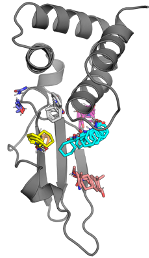
\includegraphics[width=1.5in]{ch5-suppfig1.png}
%         \caption[FTMap results for the main cryptic pocket highlighting an example protein structure and hotspots where a variety of small organic probes form energetically favorable interactions.]
%             {FTMap results for the main cryptic pocket highlighting an example protein structure (gray) and hotspots where a variety of small organic probes (multicolored sticks) form energetically favorable interactions. The probe molecules are intended to capture different drug-like interactions (such as hydrogen bonding and Van der Waals contacts) and include acetamide, acetonitrile, acetone, acetaldehyde, methylamine, benzaldehyde, benzene, isobutanol, cyclohexane, N,N-dimethylformamide, dimethyl ether, ethanol, ethane, phenol, isopropanol, or urea.}
%         \label{fig:ch5-suppfig1}
%     \end{figure}

%     \begin{figure}[!htb] %Positioning code for figure
%         \centering
%         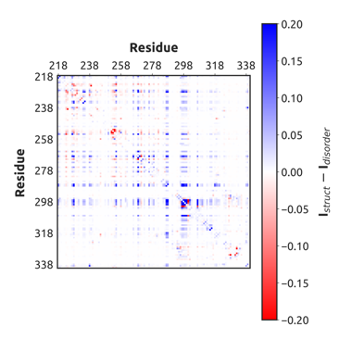
\includegraphics[width=2.5in]{ch5-suppfig2.png}
%         \caption[Purely structural correlations dominate the eVP35 allosteric network.]
%             {Purely structural correlations ($I_struct$) dominate the allosteric network identified by CARDS as they are typically greater than the disorder-mediated couplings ($I_disorder$, which includes correlations between the structure of one residue and the disorder of a second, as well as correlations between the disorder of two residues).}
%         \label{fig:ch5-suppfig2}
%     \end{figure}


%     \begin{figure}[!htb] %Positioning code for figure
%         \centering
%         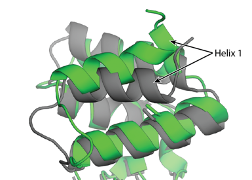
\includegraphics[width=1.5in]{ch5-suppfig3.png}
%         \caption[Motion of helix 1 sometimes exposes C247 to solvent.]
%             { Motion of helix 1 (green vs gray structures) sometimes exposes C247 (sticks) to solvent. However, the resulting pocket is small and FTMAP does not identify any hotspots in this region that are likely to bind drug-like molecules. Therefore, we focus our attention on the cryptic pocket created by the displacement of helix 7.}
%         \label{fig:ch5-suppfig3}
%     \end{figure}

%     \begin{figure}[!htb] %Positioning code for figure
%         \centering
%         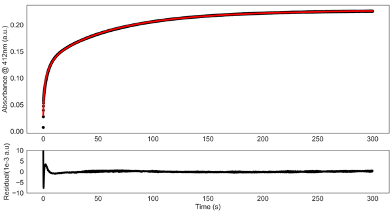
\includegraphics[width=1.5in]{ch5-suppfig4.png}
%         \caption[A representative time trace from a thiol labeling experiment ]
%             {A representative time trace from a thiol labeling experiment (black) performed at 100 $\mu$M DTNB and a quadruple exponential fit (red). The data are background subtracted (e.g. the average absorbance from three runs with DTNB but no protein were subtracted) to account for spontaneous hydrolysis of DTNB.}
%         \label{fig:ch5-suppfig4}
%     \end{figure}

%     \begin{figure}[!htb] %Positioning code for figure
%         \centering
%         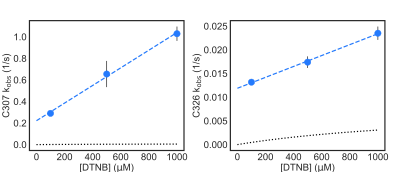
\includegraphics[width=1.5in]{ch5-suppfig5.png}
%         \caption[Thiol labeling of a C247S/C275S variant that only has cysteines in the main cryptic pocket.]
%             {Thiol labeling of a C247S/C275S variant that only has cysteines in the main cryptic pocket (C307, left and C326, right). Observed labeling rates (blue circles) are shown at a range of DTNB concentrations. Fits to the Linderstrøm-Lang model are shown in dashed colored lines and the expected labeling rate from the unfolded state is shown as black dotted lines. The mean and standard deviation from three replicates are shown but error bars are generally smaller than the symbols.}
%         \label{fig:ch5-suppfig5}
%     \end{figure}

%     \begin{figure}[!htb] %Positioning code for figure
%         \centering
%         
\includegraphics[width=4in]{ch5-suppfig6.png}
%         \caption[Observed labeling rates at 100 $\mu$M DTNB for a set of variants.]
%             {Observed labeling rates at 100 $\mu$M DTNB for a set of variants with different cysteines mutated to serines to uncover which rate in the wild-type fit corresponds to which cysteine residue. Error is standard deviation from three replicates. Dash represents rates not measured due to the absence of that cysteine residue.}
%         \label{fig:ch5-suppfig6}
%     \end{figure}

%     \begin{table}[]
%     \centering
%     \caption[Characterization of the folding/unfolding of VP35’s IID]{Characterization of the folding/unfolding of VP35’s IID used to test whether the observed thiol labeling is due to fluctuations within the native state or global unfolding of the protein. K is the equilibrium constant between the folded and unfolded state determined from denaturation data, kunfold is the unfolding rate of the respective variants measured by intrinsic tryptophan fluorescence.}
%     \label{tab:ch5-supptab1}
%     \begin{tabular}{|l|l|l|}
%     Variant     & K                     & K$_{unfold}$(s$^{-1}$) \\
%     Wild-type   & 6.57$\times$10$^{-5}$ $\pm$ 4.0$\times$10$^{-5}$ & 0.0175         \\
%     C247S/C275S & 4.01$\times$10$^{-4}$ $\pm$ 0.8$\times$10$^{-4}$ & 0.0083        
%     \end{tabular}
%     \end{table}

%     \begin{table}[]
%     \centering
%     \caption[Intrinsic labeling rates (k$_{int}$) for each cysteine residue.]{Intrinsic labeling rates (k$_{int}$) for each cysteine residue. Intrinsic labeling rates were measured using either urea unfolded variants containing only the specified cysteine, or peptides containing the specified cysteine and its surrounding residues.}
%     \label{tab:ch5-supptab2}
%     \begin{tabular}{ll}
%     \hline
%     Residue & kint$\mu$M$^{-1}$s$^{-1}$      \\ \hline
%     C247    & 0.0566 $\pm$ 0.0007 \\ \hline
%     C275    & 0.00254 $\pm$ 0.001 \\ \hline
%     C307    & 0.0290 $\pm$ 0.002  \\ \hline
%     C326    & 0.395 $\pm$ 0.02    \\ \hline
%     \end{tabular}
%     \end{table}

%     \begin{figure}[!htb] %Positioning code for figure
%         \centering
%         
\includegraphics[width=5in]{ch5-suppfig7.png}
%         \caption[RNA sequences used in fluorescence polarization binding assays.]
%             {RNA sequences used in fluorescence polarization binding assays. The sense and antisense strands were annealed in a 1:1 molar ratio}
%         \label{fig:ch5-suppfig7}
%     \end{figure}

%     \begin{figure}[!htb] %Positioning code for figure
%         \centering
%         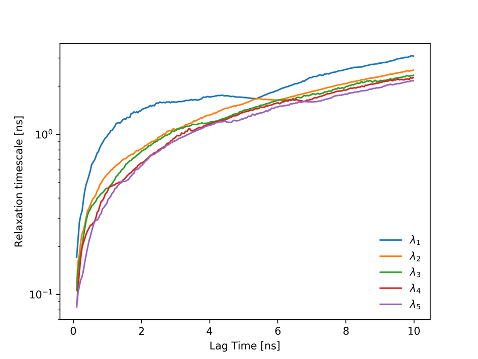
\includegraphics[width=4in]{ch5-suppfig8.png}
%         \caption[Implied timescales test for the VP35 IID MSM.]
%             {Implied timescales test for the VP35 IID MSM suggests the kinetics are stable from 3-6ns. Analysis in the main text uses a Markov time of 6 ns. Key results were consistent for lag times from 3-6 ns.}
%         \label{fig:ch5-suppfig8}
%     \end{figure}



% \bibliography{../References}
% \bibliographystyle{unsrt}
	
\end{document}